\section{The immune system and T cells}
The majority of organisms have an immune system, defined as a biological network of processes that defend the host organism against foreign pathogens and disease, that is vital for maintaining homeostasis. For mammalian immune systems, this network is broadly broken into two major arms: the innate immune system and the adaptive immune system. The innate immune system responds initially to pathogens but is limited in the molecular scope of the threats it responds to, as it uses pathogen-associated molecular patterns (PAMPs) to trigger its activity, which are generally conserved. Therefore the innate immune system responds faster but generically to pathogens - which, while useful to the host for clearing the majority of infectious agents, means the innate immune system can be overwhelmed by pathogens that may have evolved to evade innate immune system processes. It is this circumstance that creates the need for an adaptive immune system.

\begin{figure}[htbp]
	\centering
	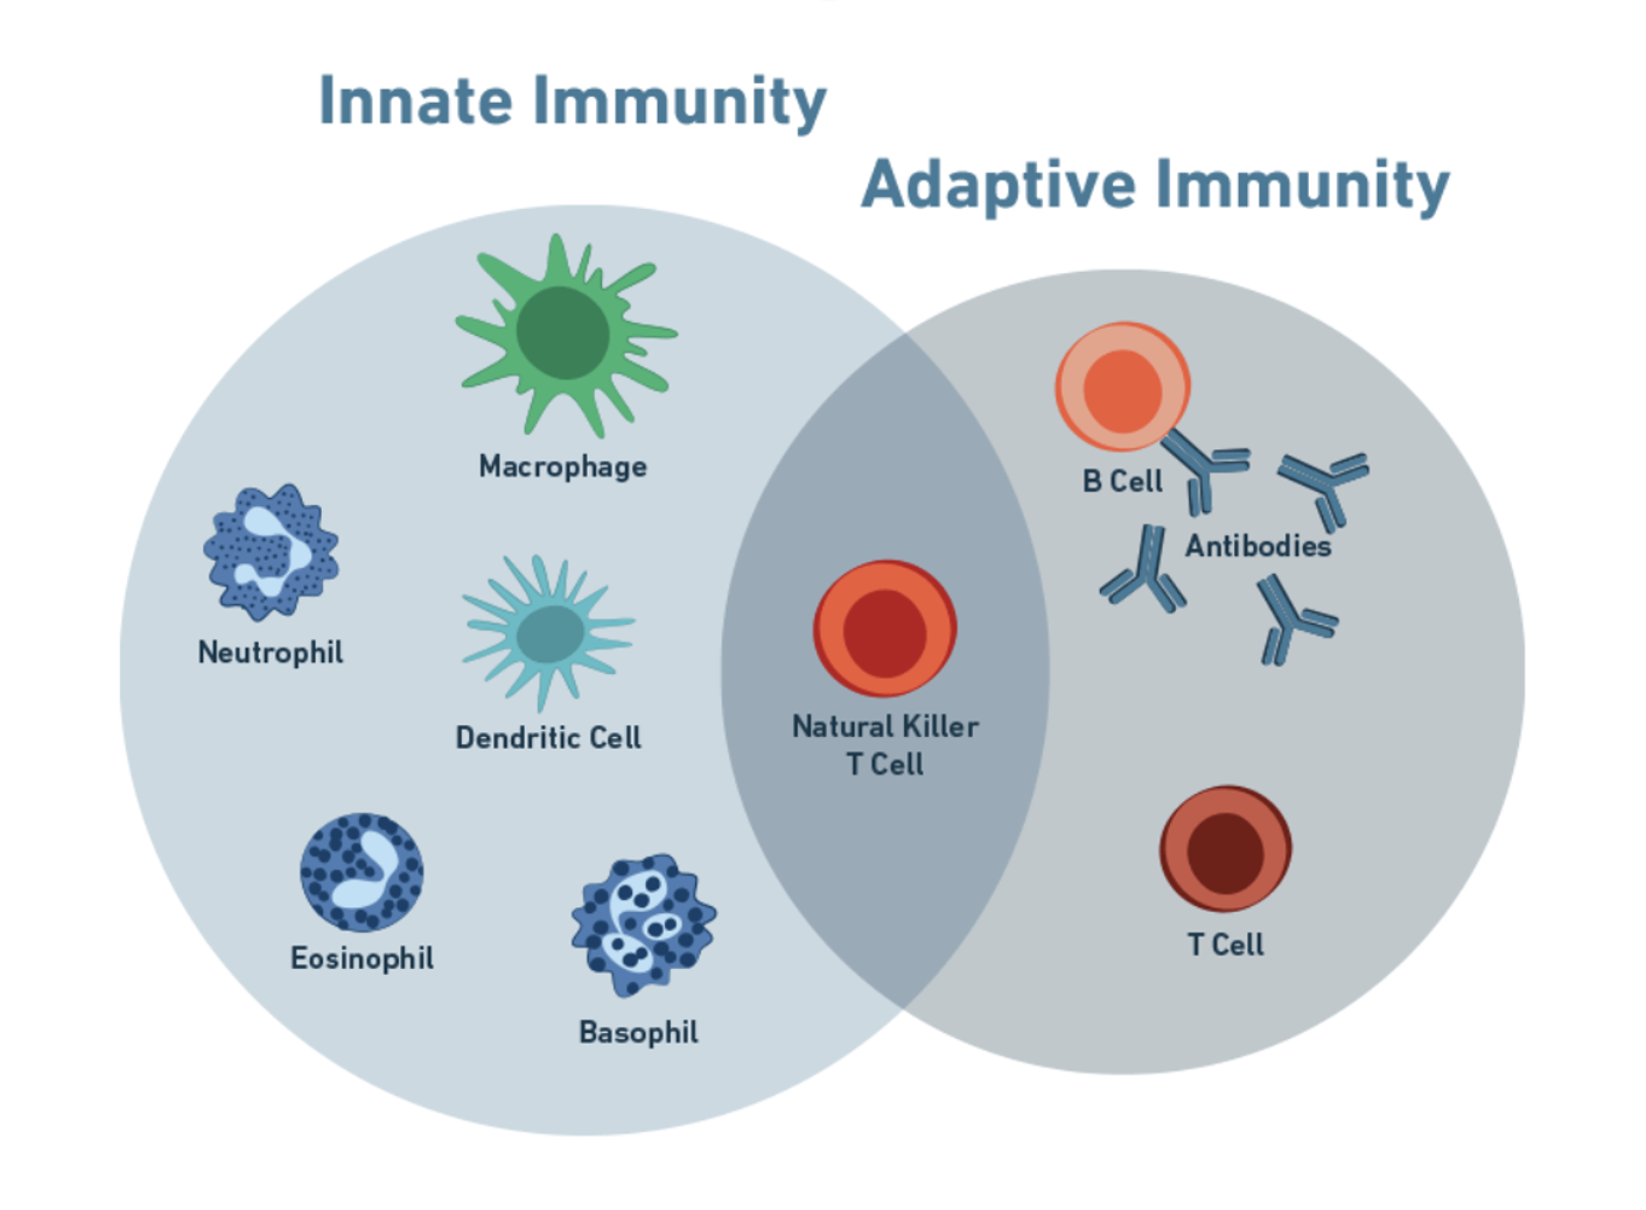
\includegraphics[width=\textwidth]{../figures/chapter1/innateadaptiveimmunesystem.png}
	\caption{Cell types of the innate vs. the adaptive immune system}
	\caption*{A Venn diagram of the immune system. The typical conception of the vertebrate immune system is typically two-armed, broken into a faster-but-general responding innate immune system (left), and a slower-but-more-specific adaptive immune system (right), of which T cells are a part of.  Almost all cell types that modern immunology research is concerned with falls somewhere within these two circles or their overlap - some immunology research is interested in characterizing certain effector or support immune cell types that fall in between innate and adaptive immunity (or can transfer their skills and interface between the two, calling into question the ontology "innate" and "adaptive" immune systems). This figure is adapted from \cite{Alam2007}.}
	\label{fig:innateadaptiveimmunesystem}
\end{figure}

The adaptive immune system responds much more slowly than the innate immune system, using this time to harvest and collect antigen and begin upramping of its antigen-specific molecular processes. The adaptive immune system is composed of two major types of cells (called lymphocytes): B cells and T cells. B cells (named for originating from the bone marrow) produce antibodies that specifically bind to antigens and identify their bound partners as foreign entities meant for destruction. T cells on the other hand (named for originating in the thymus) directly manage the cytotoxic activity of the adaptive immune system. T cells are composed of two main functional subtypes: CD8+ killer T cells (the primary focus of this thesis and heretofore referred to as any of the following: cytotoxic T lymphocytes (CTLs), cytotoxic T cells, CD8+ T cells) and CD4+ helper T cells. 

\section{T cell development}
T cells as a whole are defined by their expression of the T cell receptor (TCR), the receptor responsible for recognizing foreign antigenic peptide presented by the target cell via its Class I or Class II Major Histocompatibility Complex (MHC, or pMHC). The TCR is multi-subunit receptor that is composed of varying combinations of $\alpha$-, $\beta$-, $\gamma$-, $\delta$-, $\epsilon$-, and $\zeta$-chains, whose specific combination defines the unique sub-identity of the T cell, although the vast majority of T cells (95\%+) express the $\alpha$ and $\beta$ chains and are thus called $\alpha \beta$ T cells. There are a number of additional co-receptors that bind (either directly or indirectly) to the TCR. The most relevant to $\alpha \beta$ T cells are the CD8 or CD4 co-receptors, mentioned above. These co-receptors transduce differing signals within the specific T cell and additionally define the specificity of the $\alpha \beta$ T cell to the two different classes of MHC: CD8+ T cells bind to MHC Class I, while CD4+ T cells bind to MHC Class II. 

The ability of T cells to properly recognize and engage only with foreign antigen while ignoring self-peptides is tightly regulated and begins at a very early stage in immune system development. T cells derive from hematopoietic stem cells (HSCs) that originate in the bone marrow. HSCs then ultimately differentiate into common lymphoid progenitor cells (CLPs), which migrate to the thymus to ultimately differentiate into natural killer (NK), B, or T cells. 

The process of differentiating into T cells is primarily motivated by the need to create a functional TCR that does not react to self-antigen but does react to foreign antigen. As TCRs are made up of alpha and beta chains that are evolved to react to a wide range of possible antigens that an organism may encounter in its lifespan, T cell differentiation has been characterized in a stepwise manner that first begins with TCR-beta chain selection. T cells at this stage express an invariant pre-alpha chain called pre-T$\alpha$ that the varying beta chains (generated by VDJ recombination of the TCR-beta locus) attempt to form a stable binding partner with. Once an appropriate TCR-beta chain is identified as capable of stable binding to pre-T, the same process begins on the TCR-$\alpha$ chain against the now mature TCR-$\beta$ chain, generating a stable (but not necessarily functional) TCR.

Once a stable TCR heterodimer has been formed, the T cells must undergo a process of positive and negative selection. Positive selection involves presenting the T cells with self-antigen presented on MHC with the selection criteria of being able to bind with this complex. Those T cells that are able to bind to an MHC complex presenting self-antigen receive a survival signal, while those with TCRs that cannot MHCs do not receive this survival signal. Therefore, the body positively filters/selects for T cells with TCRs that can recognize MHCs, leaving those that cannot recognize MHCs to die off. 

After obtaining T cells that are capable of binding to MHC molecules, the next step is to select for T cells that do not auto-react to self-antigen, called negative selection. This ensures that T cells are tolerant of self-antigen and prevents auto-immunity conditions in the organism. In this stage of selection, T cells that bind to MHC presenting self-antigen and activate receive an apoptotic signal that leads to cell death. Negative selection therefore prunes the T cell population for T cells that can not only bind to MHC but do not react to self-antigen. The vast majority of thymocytes (98\%+) fail to pass positive and negative selection. Following positive and negative selection, the resulting T cell set can therefore bind to any antigen (presumably belonging to any foreign pathogen) so long that the antigen is distinct from the body’s self-antigens. 
After these stages of T cell development, these T cells (called naïve T cells) then exit the thymus and begin to circulate in the host, where they will spend their time surveying the host for disease and foreign antigens.

\section{TCR activation and downstream signaling}
If a CD8+ T cell engages an infected cell presenting foreign peptide, the T cell will initiate a cascade of antigenic-specific intracellular signaling events. Upon ligation of the TCR to the pMHC complex, the CD3 proteins (CD3$\epsilon \gamma$ and CD3$\epsilon \delta$ heterodimers and a CD3$\zeta$ homodimer) bearing ITAM (immunoreceptor tyrosine-based activation motif) also bind to the TCR.  The ITAMs on the CD3$\zeta$ get phosphorylated, so that cytosolic signaling proteins can bind to phosphorylated ITAMs and propagate the signal from the triggered TCR further downstream into the T cell. CD3$\zeta$ contains three ITAMs, while CD3$\delta$, CD3 $\gamma$, and CD3$\epsilon$ all only contain one ITAM. The CD3 chains are needed as the cytosolic tail of the TCR is extremely short and structurally do not support significant adaptor features for signal amplification molecules. This modularity also allows for an increased range of TCR signaling for fine-tuning key features of the T cell effector response (e.g. killing, proliferation, signaling, cytokine secretion) in response to a number of diverse inputs such as antigen strength, lifetime of interaction, and number of bound-TCRs at the IS.

The phosphorylated CD3 ITAMs recruit the protein tyrosine kinase Zap70 that binds to the phoshorylated tyrosine motifs via its SH2 domain.  This brings Zap70 closer to CD8-bound Lck, which further phosphorylates Zap70, activating Zap70. Upon Lck-mediated phosphorylation of Zap70,  Zap70 itself phosphorylates and activates the transmembrane protein called linker for activation of T cells (LAT). LAT acts as a scaffold, providing binding sites for a number of signaling molecules (via its own phosphorylated sites) that link these signaling molecules, including the lymphocyte cytosolic protein 2 (SLP76) which provides even further additional binding sites, on the LAT signaling complex, SOS,  Grb2, Itk, Vav, Nck1, and Fyb, in space and time.  

One of the most crucial signaling molecules that binds to LAT is the protein phospholipase C$\gamma$1 (PLC$\gamma$), which generates key lipid secondary messenger molecules. Phosphatidylinositol 4,5-bisphosphate (PIP2) is an input to PLC$\gamma$ function. Once phosphorylated and activated by Itk, PLC$\gamma$'s enzymatic activity (using PIP2 as a substrate) generates two products: diacylglycerol (DAG) and the soluble inositol 1,4,5-trisphosphate (IP3). Diacylglycerol accumulates in the IS, which prompts recruitment of the microtubule motor protein dynein and drives polarization of the microtubule-organizing center (MTOC) \cite{Quann2009} and the recruitment of lytic granules to the immune synapse (further discussed in the T cell degranulation and target cell death introduction section \cite{Stinchcombe2006}. IP3 is soluble and diffuses throughout the cytosol, eventually binding to its receptor inositol trisphosphate receptor (InsP3R), located on the endoplasmic reticulum (ER). The binding of IP3 to InsP3R triggers release of calcium ($Ca^{2+}$) ions into the cytosol, initiating calcium-dependent transcription programming. These include the NFAT, NF-$\kappa$B, and AP1 signaling pathways, all of which assist in fully activating the T cell. Another notable lipid secondary messenger is phosphatidylinositol (3,4,5)-trisphosphate (PIP3). PIP2 is phosphorylated by the phosphoinositide 3-kinase (PI-3K) to give PIP3, which further activates downstream signaling proteins, most notably Akt, which is highly involved in T cell metabolism.

The generation of spatial gradients and patterns of lipid secondary messenger molecules at the plasma membrane is highly consequential, resulting in the formation of a necessary killing and major signaling structure called the immune synapse. 

\section{The immunological synapse and the T cell cytoskeleton}
The immunological synapse (also called the immune synapse) is the highly organized, structurally stereotyped interface that T cells form against an APC. It is classically characterized as a concentric, annular structure that bears a "bulls-eye" center surrounded by a ring of filamentous actin (see Figure \ref{fig:immunesynapse}, left). The immune synapse is a major T cell signaling and killing megastructure, and robust formation of the immune synapse is essential for the T cell to achieve its maximal cytotoxic efficacy, in particular when concerned with lytic granule secretion \cite{Ritter2015}.

\begin{figure}[htbp]
	\centering
	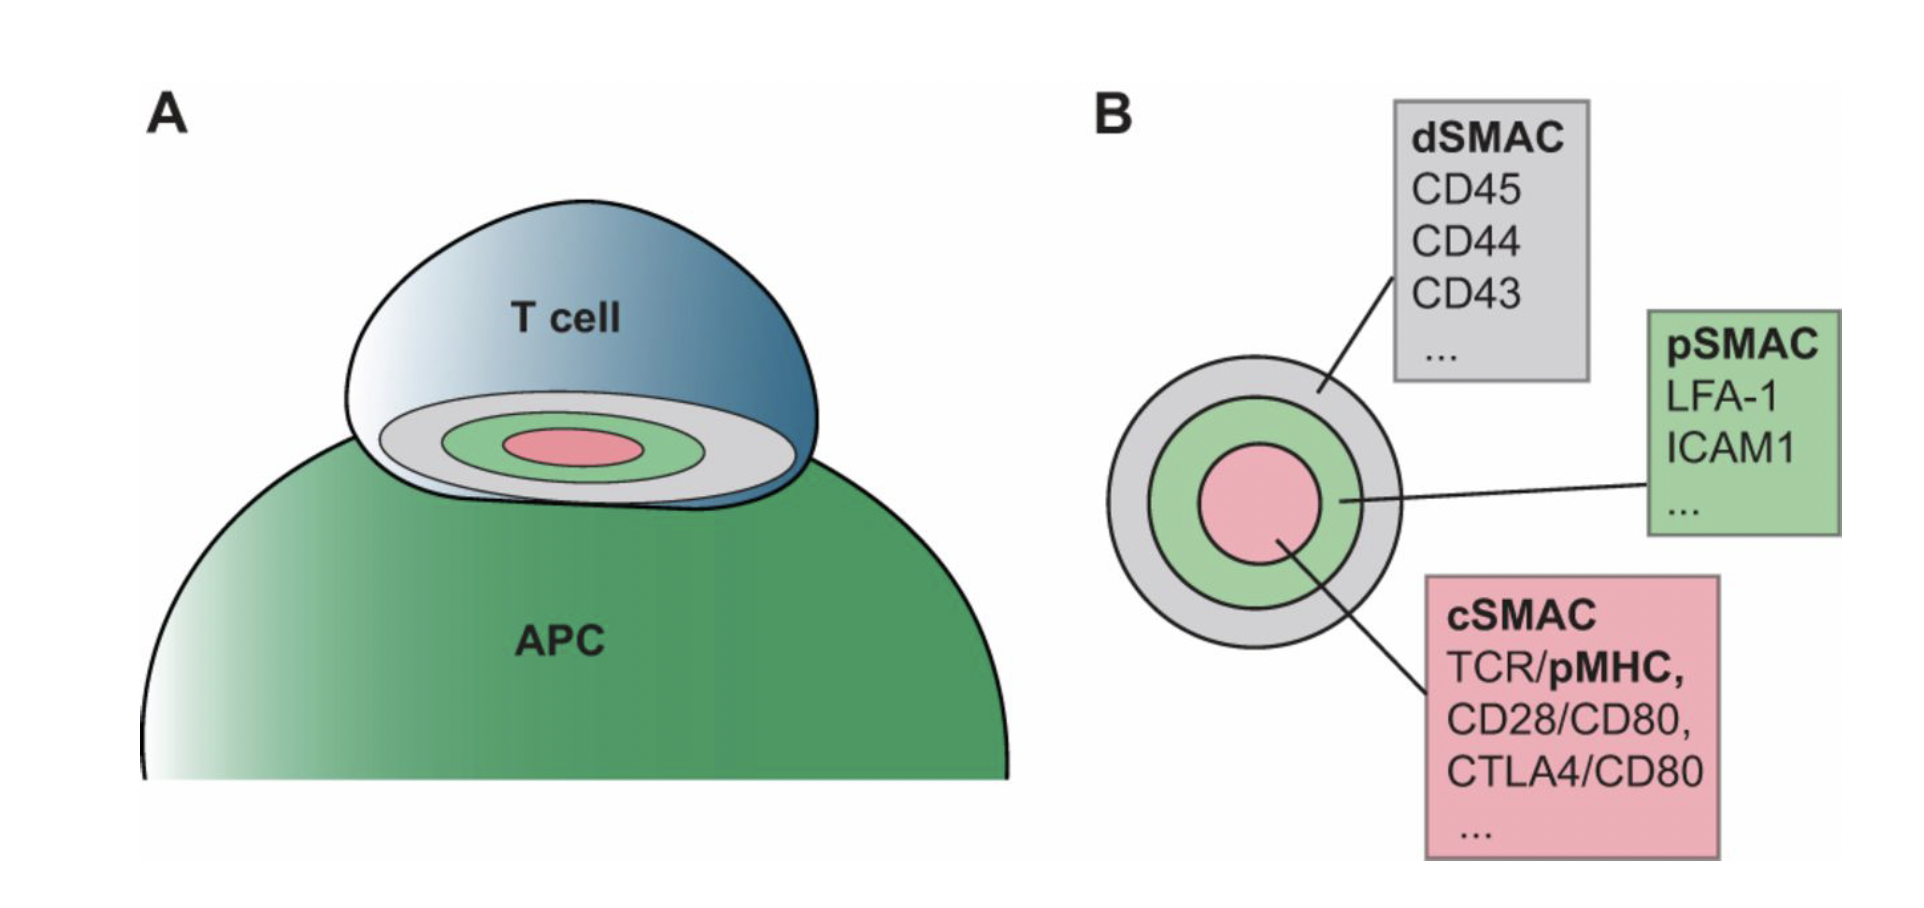
\includegraphics[width=\textwidth]{../figures/chapter1/immunesynapse.png}
	\caption{The immunological synapse}
	\caption*{\textbf{A}: A schematic of the canonical model of the immune synapse. The T cell (blue, above) is in contact with the APC (green, below). The IS is shown as a series of interfacial concentric rings.  \textbf{B}: The IS is classically divided into three regions, extending from the center outwards: the cSMAC, the pSMAC, and the dSMAC.  The proper formation of the IS results in functionally distinct and biochemically patterned regions.  This figure is adapted from \cite{Yu2013}.}
	\label{fig:immunesynapse}
\end{figure}

The 
Actin cdc42 Rho RacGTPases signaling etc !

dSMAC
pSMAC
cSMAC


\section{T cell degranulation and target cell death}
The killing mechanism of CTLs is fundamental to robust anticancer and antiviral responses.  CTLs achieve their cytotoxic effects by managing a two-pronged approach 1. specifically destroying only infected or oncogenic target cells (recognized via ligation between the TCR and its specific pMHC interaction) and 2. preserving the integrity of the surrounding healthy bystander tissue. 

The T cell has evolved countless mechanisms in order to balance this dual mandate. The most prevalent mechanism of T cell-mediated killing of target cells involves the secretion of the hydrophobic protein perforin and granzyme proteases, called degranulation \cite{Dustin2010, Stinchcombe2007}. When released, perforin oligomerizes in a calcium dependent manner \cite{Law2010} and forms pores on the target cell surface, (around 16nm in diameter) \cite{Cartwright2014}, inducing significant membrane damage. The target cell responds to this traumatic event at the plasma membrane using a mechanism that permits granzymes entry to the cytoplasm, where they cleave apoptotic substrates that induce apoptosis \cite{Keefe2005}. Because all cell types are capable of being killed and cleared in this way (that is to say, both infected and healthy cells),  specialized mechanisms have evolved over time in immune cells to ensure that the effects of perforin and granzyme are constrained to the target cell alone.  

This calcium flux is a required step for lymphocyte degranulation, which is (ORAI1-mediated calcium influx is required for human cytotoxic lymphocyte degranulation and target cell lysis)

Cytotoxic T lymphocytes store their perforin and granzymes in specialized secretory lysosomes called lytic granules (0.5 to 2 $\mu$) \cite{Sanchez-Ruiz2011}, whose acidic pH environment quenches the lytic and apoptotic activity of both proteins \cite{Thiery2014, Keefe2005}. Following mere minutes of target cell recognition, the lytic granules are trafficked along microtubules to the immunological synapse (IS). At this site, they fuse with the plasma membrane, releasing their contents into the intercellular space. At the same time,  F-actin and the associated actin nucleation promoting factors (NPFs) at the IS undergo significant spatiotemporal remodeling.  This results in a highly complex landscape of highly dynamic actin sheets and protrusions \cite{Ritter2015}. Canonically, actin clearance from the center of the immune synapse (cSMAC) is required for fusion of lytic granules to the center of the synapse \cite{Ritter2015}, although newer models of degranulation highlight the need for transient actin polymerization at the site of degranulation to potentiate the pore forming effects of perforin \cite{Tamzalit2018}. This is related to T cell mechanical force exertion against the target, which significantly amplifies T cell effector function \cite{Tamzalit2018}.

\section{T cell mechanical force exertion}
Immune cell-immune cell interactions are typically described as a series of interrelated biochemical receptor-ligand signaling processes (and this introduction has done the same). While this characterization is not incorrect, it ignores the mechanical dimension of immune cell interactions, which have been identified as a significant hubs of cellular decision making. Immune cells have been demonstrated to have a number of biophysical sensing functions, including cancer cell surveillance and immune cell function and cytotoxicity.

The CTL immune synapse has been shown to be a physically dynamic structure, capable of exerting force against a resisting target or surface and 

Some recent studies demonstrate that the actin-rich structures formed during T cell adhesion and degranulation are actually involved in boosting the lytic activity of perforin by dynamically applying mechanical force against the target cell \cite{Basu2016, Tamzalit2018} and sensitizing the target cell to perforin insertion, which must overcome the hydrophobic interior of the plasma membrane in order to pierce the target cell plasma membrane and trigger cell lysis.

Recent work has provided insight into how the TCR can distinguish
single amino acid substitutions in short peptides. Previous research has
shown that the $\zeta$-chain of the TCR undergoes conformational changes to
expose phosphorylation sites in its ITAM domains67. Other work has shown
that the TCR is an anisotropic mechanosensor that requires force orthogonal
to the IS for the induction of calcium signaling68. The model that these two
observations suggest is that force is required to expose ITAM domains on the
TCR, which leads to the induction of membrane proximal signaling.
Furthermore, the TCR-pMHC interaction has been shown to function as a
catch bond69. A catch bond is a type of bond in which application of a force
increases the lifetime of the interaction. It was shown that the capacity to form
a catch bond plays a critical role in enabling the TCR to discriminate between
high and low affinity agonists69. Together these studies demonstrate the
important role of mechanobiology in TCR activation and signaling.
The IS has been shown to be a dynamic and physical structure that is
capable of exerting mechanical force70,71. Naïve T cells have been shown to
exert mechanical force on polydimethylsiloxane (PDMS) pillars coated with
activating proteins71. It is conceivable that T cells could exert forces as a way
of sensing the mechanical properties of activating surfaces. This is supported
by previous research demonstrating that T cells are more strongly activated on
softer rather than stiffer PDMS surfaces, as measured by cytokine production
and proliferation72. Activating peripheral blood mononuclear cells (PBMCs) on
softer surfaces with CD3/CD28 antibodies tended to increase shedding of
CD62L, which is a consequence of T cell activation72. This is intriguing
19
because the opposite phenomenon has been observed for naïve mouse T
cells activated on polyacrylamide surfaces with CD3/CD2873. Possible
explanations for this discrepancy include a difference between human and
mouse cells. It is also possible T cells respond differently to antibodies on
PDMS and polyacrylamide surfaces. Further research is needed to understand
the precise role of surface tension on T cell activation. Yet, these studies are
intriguing and support the concept that signaling and cell biology are not
merely biochemical reactions. These observations show that mechanical
properties of biology are important factors that have been largely overlooked
in immunology until recently.


\section{Thesis Aims}
The further successful development of immune cell therapies thus far has been and will continue to be dependent on a deeper understanding of basic T cell effector function. To this end, this thesis is chiefly focused on a molecular approach to studying the mechanotransduction of T cell effector function and the dynamic relationships between its biophysical and biochemical dimensions. The results of this study are broken across two chapters, whose contents are summarized below.

While it was known that the CTLs use physical force to amplify the pore-forming effects of perforin and resulting positive correlation between force exertion and  target cell death, it was unclear what cellular structures T cells form in order to actualize this force against the target cell membrane and manipulate this relationship. It was also unclear what proteins or molecules were involved in this membrane perturbation/distortion process. Chapter 2 of this thesis will address the results of the experiments testing these outstanding questions through the use of pharmacological and genetic perturbations against the actin nucleation promoting factors (NPFs) Wiskott–Aldrich Syndrome protein (WASP) and WAVE2 (WASP-verprolin homolog 2) that directly affected T cell force exertion, and studying their resulting cytotoxic capabilities and dynamics via co-culture assays and imaging.

Another outstanding question arose from the observation that T cells degranulate specifically near areas of synaptic force exertion. While this dovetails with the observation that force exertion amplifies the pore-forming effects of perforin (as discussed in the Introduction and Chapter 2), it was unknown what types of forces or interactions coordinated these two phenomena of degranulation and synaptic force exertion so that they could be unified in space and time. It was also unknown what force-sensitive molecules could be mediating this intercellular communication. Chapter 3 addresses the study conducted to address these questions, which also used pharmacological and genetic perturbations against integrins (primarily lymphocyte function-associated antigen 1, or LFA-1) on T cells in order to modify the force output of these T cells and change their degranulation and cytotoxic behavior as observed through co-culture assays and unique and creative imaging experiments. Altogether, this thesis aims to clarify the specifics of the T cell killing event (encompassing T cell force exertion and degranulation) in order to better inform future T cell studies and therapy design.
